\section{Communication Tips}

The role of verbal communication is critical for bureaucrats. 
There is a lot of advice on effective communication (enunciate, speak loud enough to be heard, be humble, be curious), so the advice below is highlighted because of prevalence in bureaucratic organizations. 
The following is generic to interactions outside of bureaucracy. 

For general writing tips, see Strunk's and White's Elements of Style and other resources \footnote{\href{https://www.youtube.com/watch?v=vtIzMaLkCaM}{LEADERSHIP LAB: The Craft of Writing Effectively} and \href{https://www.youtube.com/watch?v=aFwVf5a3pZM}{LEADERSHIP LAB: Writing Beyond the Academy}}.

\subsection*{Tip: Not all interaction challenges are communication problems.}
Sometimes an inability to discuss ideas is not a communication problem but a psychological deficit of personality. Distinguishing ``I'm an ineffective communicator'' from ``the person I'm talking with doesn't communicate effectively'' from ``that person has a diagnosed psychological reason they are unable to communicate'' is tough for those of us who are not psychologists or psychiatrists. 

%how to measure effectiveness: The waste or inefficiency in a bureaucracy is a measure of the lack of coordination or inconsistent decision making among the members

\subsection*{Tip: Avoid relying on stereotypes.}
Within an organization different teams may build up reputations for certain behaviors, or there may be significant events that the team is associated with. 
When interacting with members of a team that has a reputation, avoid relying on that stereotype or event as an opening for discussion. 
You're speaking to an individual, so address that person's behavior.



\subsection*{Tip: Avoid questions that have a binary response\label{sec:yes_no_questions}.}

Responding to a request with ``no'' is advantageous for the person replying to the question. There is less work required, less risk of failure, and better continuity. As an example of a poorly framed question, I could ask, ``Can I have a copy of the data you're using?'' The person I'm asking is less disrupted if they refuse to share. 

A more constructive phrasing is ``I need information on X to work on Y, and I think you have information about X. How can you help me get information on X?'' By clarifying my intent, I allow the person with the data to provide options I may not have considered.

Similarly, when I'm being asked for information, I try to learn the person's intent motivating the question. Sometimes the requester doesn't actually know what to ask for. Instead of ``no'' I try to figure out how to enable the person to be successful. 

\subsection*{Tip: Leverage the other person's experience while focusing on your own\label{sec:advice}}

Advice without context is less effective.\\
\textit{Bad}: ``Here is what I think you should do in that situation.''\\
\textit{Better}: ``Here is what I did in that situation.''

People usually find talking about themselves an easy topic if you are curious about their experiences. 
If you can learn the other person's background and history and motivations, you can weave that into the advice you provide. 
Tailoring your message increases the likelihood of implementation. 

\subsection*{Tip: Avoid Platitudes\label{sec:platitudes}.}
% https://graphthinking.blogspot.com/2017/10/why-platitudes-are-used.html
\href{https://en.wikipedia.org/wiki/Platitude}{Platitudes} are \gls{thought terminating}; the statement feels true and is resistant to debate. Platitudes capture a feeling with sufficient accuracy, but with imprecise language. As a result, there's no specific action.

Because platitudes result in a conclusion, the conversation participants may feel more bonded. However, that bond is shallow.

Example platitudes to avoid:
% https://graphthinking.blogspot.com/2017/02/phrases-which-serve-as-thinking-stoppers.html
% https://graphthinking.blogspot.com/2017/10/a-list-of-platitudes.html
\begin{itemize}
    \item pick your battles
    \item Some things you can't explain
    \item Your time will come.
    \item You can be anything that you want to be
    \item I just want to get through this day
    \item It is what it is
    \item I'm just one person
    \item That's that
    \item Life's not perfect
    \item Life's not fair
    \item There's only so much you can do about it
    \item What is meant to be will be
    \item It is God's will
    \item It's part of God's plan
\end{itemize}

If your goal is to understand a concept or issue deeply, you need to use precise language.

\subsection*{Tip: Strive to use Precise Language}

Imprecise language causes miscommunication. Intent is unclear, as is expected consequence.

If you have a specific definition for a word central to the topic of interest, ask your new collaborator for their definition. Do not expect others to share your definition even when there are established norms for the topic. 

Instead of asking a collaborator, ``Are you taking action on this topic?'' ask ``What actions are you taking on this topic?''

If someone claims, ``We plan to get to that action,'' ask for a timeline. A deadline can be for an artifact or a re-evaluation of the topic.

In the short-term imprecise language takes less work to create and can take less time to convey. 

The importance of precise language is proportional to the potential consequences of action/inaction/wrong action.
Precision also should be proportional to the complexity of the topic being discussed. 

\subsection*{Tip: Word is bond\label{sec:word-is-bond}}

Your communication (verbal, written) is your reputation. People rely on what you tell them even if there isn't legal recourse. Reliance on your word is why precision matters. 

Frustration and disappointment follow when you don't uphold your word, or others misinterpret your imprecise language, or you are misunderstood.

Communication implies responsibility for the content.  There is a corresponding accountability in the relationship between speaker and listener (or writer and reader).

\subsection*{Tip: Take care near the boundaries of knowledge}

Trying to find someone else's extent of knowledge is tricky -- they don't want to appear stupid. They may interpret the exploration at a trap. ``I don't know'' can be an embarrassing statement to make, even if you don't share their embarrassment. 

Knowing the limitations of your own knowledge and disclosing those boundaries to others is critical. Distinguish what you know from speculation about things you don't. 

\subsection*{Tip: Listen all the way to the last word of the speaker}

Formulating a response to the first part of an idea or a sentence is tempting. Waiting for the speaker to finish before thinking of how to response is courteous. Waiting creates a pause which makes you seem more thoughtful. 

This is complicated by the speakers who include long pauses for contemplation and then resume. 

\subsection*{Tip: Eliminate speaking over other people.\label{sec:crosstalk}}
% https://graphthinking.blogspot.com/2017/10/crosstalk.html

Crosstalk occurs two people who are communicating verbally experience interference from another audible conversation. That can occur because a third person is talking at one of the original two participants, or when four or more people are holding two separate conversations concurrently. 

Crosstalk in a bureaucracy is motivated by
limited time available to communicate. A meeting participant may feel inspired by something someone else said and want to interject. 
%Typically manifests as popcorn style stories based on experience. 
%Intended as wisdom for self-validation by others in our community. 
Crosstalk can indicate engagement and enthusiasm, or it can be due to the speaker wanting to dominate the topic through interruption. The likelihood of crosstalk is dependent on the level of aggressiveness of participants.
In either case (enthusiasm or power-seeking), the original speakers are disrespected. The original speaker may feel annoyed at being interrupted.



%Crosstalk has four roles and a minimum of two people participating: the discussion facilitator, the original speaker, the interrupter, and other meeting participants. 
%During crosstalk, the discussion facilitator loses control of the interaction to the interrupter.  
The audience is frustrated by the lack of clarity of where to focus. This distraction causes participants to lose of focus and productivity of the interaction decreases.

Bystander intervention for out-of-control meeting: raise your hand. \marginpar{[Tag] Actionable Advice} This non-verbally reverts focus back to the discussion facilitator. 

\subsection*{Tip: Account for Warnock's dilemma}
% https://graphthinking.blogspot.com/2018/09/dealing-with-warnocks-dilemma-in.html
\href{https://en.wikipedia.org/wiki/Warnock\%27s_dilemma}{Warnock's dilemma}
is the common experience of figuring out how to interpret not getting feedback. This is especially vital in meetings where the speaker or facilitator needs to gauge participant comprehension of delivered content. Simply asking ``Does anyone not understand what I just described?" is likely to get no response from attendees because individuals want to avoid looking stupid.

\ \\
\textit{Technique}: Pick an individual to provide a recap.\\
\textit{Technique}: Survey the audience using multiple choice to gauge understanding.\marginpar{[Tag] Actionable Advice}

\subsection*{Tip: Seek action with a deadline}

% https://graphthinking.blogspot.com/2017/11/collected-wisdom.html
When asking someone for help or input, specify a deadline for their response. \marginpar{[Tag] Actionable Advice}This helps the person prioritize their tasks.

\subsection*{Tip: Identify the cause of miscommunication}

% https://graphthinking.blogspot.com/2019/06/miscommunication-versus-inability-to.html
\begin{itemize}
    \item miscommunication the cause is often due to definitions of words used or differences in context. In this situation, additional time spent communicating and taking different approaches is sufficient to remedy the issue.
\item A speaker may be inarticulate. If the speaker is unable to coherently convey their internal experience to a listener, then the communication failure is of a distinct category. No amount of additional communication will lead to improved understanding on the part of the listener.
\item A speaker simply has nothing to say about a subject. Regardless of whether they are capable of articulating a concept, they may be unable to relate to the topic. Often a person in this situation still wants to participate, but they are unable to meaningfully contribute. 
\end{itemize}
% https://graphthinking.blogspot.com/2019/05/identifying-empty-talk.html
Empty talk is the use of words that are ill-defined, emotionally resonant, inactionable, and impersonal.

\subsection*{Tip: ask-tell-ask}

Collaborating with fellow bureaucrats who have expertise in areas you do not requires extra work. There may be differences in the words used to describe certain situations, more precision in wording that you're used to, or thinking about situations in ways you are not familiar with. In that context, to bridge the differences you can ask, tell, ask\footnote{\href{https://cepc.ucsf.edu/sites/cepc.ucsf.edu/files/Curriculum_sample_14-0602.pdf}{``The 10 Building Blocks of Primary Care: `Ask Tell Ask' Sample Curriculum''} and \href{https://www.the-hospitalist.org/hospitalist/article/125126/qi-initiatives/ask-tell-ask-simple-technique-can-help-hospitalists}{Ask-Tell-Ask: Simple Technique}}. 

The first step is asking what the other person's perspective is on the topic. This helps establish the appropriate level of nuance is and can tell you how that person frames the issue. The second step is to tell the person what you want to say. The ``tell'' step should leverage what you learned from the first ``ask'' step. Use phrasing that is consistent with what you just learned from the other person. The third step is to ask the person what they heard from you. If they are unable to tell you, you may need to refine your delivery. To improve the likelihood of success keep the content in the second step short. 

The ask-tell-ask technique can be used iteratively in the same conversation, especially in discussion complex topics with a new collaborator. \marginpar{[Tag] Actionable Advice}Using ask-tell-ask takes long than just telling but increases the effectiveness of the communication. You also get to learn more about the other person's perspective. 


\subsection*{Tip: Initial responsiveness and status updates}
In a bureaucracy requiring approval, or soliciting input, sometimes waiting can provide value to the person doing the waiting. The request may be overcome by events, or the person asking may remind which indicates priority.

\subsection*{Tip: Make deadlines explicit}

Typically requests have two deadlines. The first deadline is when a response is sought. The second deadline is when a response is no longer useful.  

As an example, suppose I am inviting people to a meeting. I send the invitation 5 days prior to the meeting and I want to know who is able to attend by 3 days before the meeting. The second deadline is the time of the meeting. Replies after that second deadline do not help me understand who is going to attend. 

\subsection*{Tip: Read each email/memo/report to determine the purpose }
% https://graphthinking.blogspot.com/2021/03/read-each-email-to-determine-purpose.html

\textit{Problematic behavior}: scan the text of a message, see if there is immediate action or response needed. If no action or response is needed, go to the next email. \\
 That does not work for emails that contain logistics associated with future events. 

Instead, consider possible intentions of the person writing the email. 

\textbf{Decision needed}. Typically includes context. \\
\textit{Action}: if the team maintains a decision log, update that.
Response is selection of a choice.

Tip: Instead of asking for a decision, ask for if the person is opposed.

Tip: instead of asking for a decision, ask for the go-ahead. This framing biases the respondent towards action (specifically approval) rather than thinking. 

\textbf{Situational awareness}.\\
\textit{Action}: Expected default is no action, but interject if there's an issue.


\textbf{Action or Tasking}.\\
\textit{Action}: Do something within some deadline

\textbf{Approval sought}.\\
\textit{Action}: Confirm or deny

\textbf{Feedback sought}.\\
\textit{Action}: Assessment of proposal


\textbf{Meeting logistics}. Can be an announcement (widely available), registration (limited attendance), or invitation (specific to you). Attendance is optional or require. \\
\textit{Action}: Create or update a calendar event
Response should restate the logistics (time/date/location/purpose) to confirm. 

\textbf{Brainstorming}\\
May provoke a response for building on an idea.
``For your situational awareness, no action needed." Notification of activity by someone else. Or change in plans. 
If needed, a correction to the described direction might trigger a response or even a meeting.

\textbf{Reference} e.g. describing a process or business workflow. Or a citation.\\
\textit{Action}: Copy process documentation to wiki. Copy citation to bibliography.
Acknowledgement response thanking the sender for the update/clarification.

\textbf{Setting a formal policy or issuing an informal edict}\\
\textit{Action}: move the policy/edict documentation to Confluence or Wiki
Acknowledgement response needed only if the edit is aimed at just me or the group I am leading

\textbf{Question}\\
If this is a recurring question, move to a ``Frequently Asked Questions" page on Confluence or Wiki.
Response needed that provides answer or seeks clarification.


Here I'm using ``action" to refer to activities outside the email channel. 

If I read email to figure out the purpose of the email, that will help me determine what action and response are relevant. 

Whether I am the only recipient or on of many receivers can change the intent of the email, and whether I'm in the ``to" or ``cc" field matters. Unfortunately, ``to" versus ``cc" are not reliable indicators since email senders do not reliably conform to the expected use. 



%This categorization of text within emails is a useful natural language processing challenge for machine learning. Currently a few email providers already do some of this with identifying meeting logistics, providing reminders to follow-up, and providing reply snippets. A browser plug-in that differentiates the various purposes of text could help readers determine relevant actions and responses. 

An email sent to multiple recipients may have different purposes for different readers. The reader's role or knowledge may factor into how they interpret the content. The inclusion or exclusion of recipients alters how the content is understood. 

\subsection*{Tip: Don't seek attribution for contributions; credit others\label{sec:credit-others}}

Give credit to others for good ideas and beneficial actions. Either they accept credit and you are seen as a contributor to their success, or they push back and you look generous. Credit is not a \href{https://en.wikipedia.org/wiki/Zero-sum_game}{zero sum game}.

\subsection*{Tip: Offer to take blame\label{sec:take-blame}}

Before an action commences, tell collaborators that you are willing to accept blame if something goes wrong. This alleviates their fear of risks.

\subsection*{Tip: Survey stakeholders}
% https://graphthinking.blogspot.com/2016/01/how-to-solve-and-not-solve-problems.html

Suppose you are a \href{http://www.peacecorps.gov/}{Peace Corps} worker in Africa. You show up and the village doesn't have easy access to clean water. Villagers walk a long ways in dangerous areas for dirty, unsafe water. This is a very obvious problem and all the villagers agree that they don't have good water and that this problem should be fixed.

Implementing the solution would take about a week - get the equipment to the village, drill a well, build a pump.

You could take additional time and involve the villagers in this project. They could participate in getting the equipment, which should lead to a sense of ownership.
But then when the equipment shows up, they don't take action to drill the well. If the well is drilled, it soon falls into disrepair and the villagers are back to doing things they way they used to. What happened?

The villagers don't see access to clean water as the most significant issue. You came in and imposed your view of what the problem is and how to fix it. When you impose your view of what the problem is, the solution won't be adopted by villagers because they don't prioritize it.
It is better to survey the community to see how they operate. What do they think the problems are?
Both leadership and the community members need to provide priorities.

This issue is exacerbated if you come to the village as a representative of a company providing wells. You are biased when you ask, ``Do you have any problems?"

Of course the villagers have water problems which could be fixed with better wells. However, when you get into the details of placing or improving a well, they lose interest. What the community really wants is free installation, zero maintenance, easy to use, and no operational costs. That would improve their life.

When you say there's cost (both initial investment of capital and then operations/maintenance) and a learning curve associated with the solution, then the user's interest wanes -- you are presenting another cost/benefit ratio for them to evaluate. Then they ask ``Can we get by without the well?" Yes, they don't need the well -- they've survived without it.

Novel solutions (in this example, drilling a well and installing a pump) have barriers to adoption. Two barriers are the current priorities of the community and the incumbent solution/processes.

If there are problems with higher priority, the community will delay implementing your solution. That's fine if the higher-ranked priorities are bounded, but they are often not. An example of this is the following:
Suppose a person has three tasks, and you introduce a solution which is a fourth task.
If the first task is ``go from point A to point B," then that task will eventually be eliminated and there will be three remaining.
If the second task is ``secure your village," that is an unbounded task. The person won't get to or won't prioritize your low-ranked task.

How will your solution impact their higher-ranked priorities?

\ \\

\subsection*{Email Structure\label{sec:email-structure}}

% from https://graphthinking.blogspot.com/2021/10/structuring-email-content-for.html

If implementing all these tips sounds like a lot of work, that's because it is. Effective written communication requires intentional effort because of the lack of augmenting channels (compared to voice or video or in-person). 



Use consistent design and structure for your emails. Emails are part of your professional reputation.

Emails start with a greeting: Hi, Hello, Good morning, Good afternoon, Good evening. 
Email greetings include the name of the targeted recipient(s). 

Emails terminate with a professional closing, e.g., ``Kindly", ``Regards", etc

Emails contain a signature block with contact information -- phone number, normal hours of response, which timezone you're in if your team spans timezones, how long to wait for a response before asking again, which communication channel I prefer, etc.

\begin{figure}
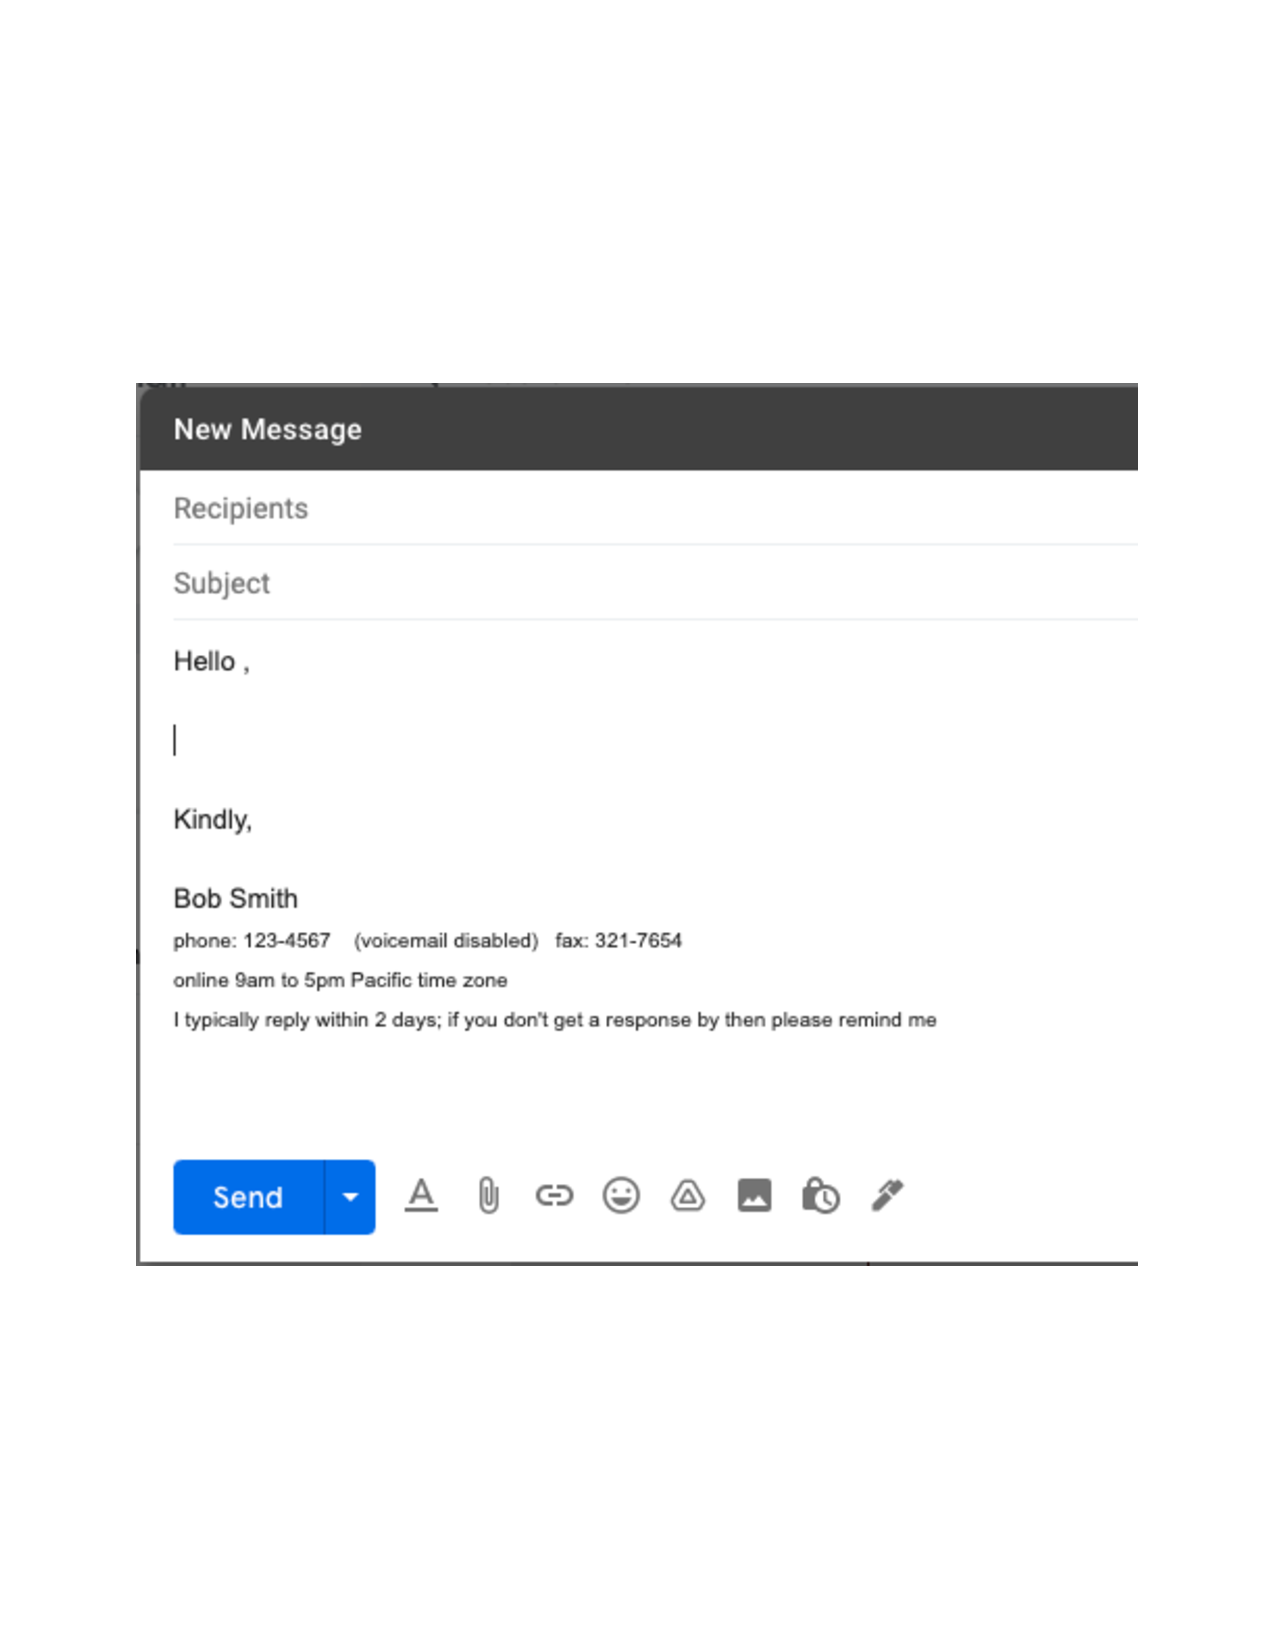
\includegraphics[width=1\textwidth]{images/email_template.pdf}
\caption{Template for new email messages. Greeting has a space after the comma -- that is where the recipient's name will go. Signature block uses smaller after the name.}
\label{fig:email_template}
\end{figure}

Email signature blocks do not include unnecessary images, as that uses more storage for recipients. 
Email threads focused on a specific instance of a recurring event include the date (YYYY-MM-DD) in the subject line. 

Based on the purpose of the email, example key phrases for subject lines include: ``meeting notes" versus ``agenda" versus ``question about".

Revising an existing subject line can disrupt the ability of email software to thread conversations. However, sometimes the revision is worth breaking threading.

When replying to an ongoing thread, retain the original message as part of the thread to provide readers historical context.

When replying to threads with sensitive messages, sanitize the included content as appropriate by removing name or identifying details.

If an email contains multiple requests or questions, at the top of the email (after the greeting) explicitly say how many of each type. Then, in the body of the message, number them.

\begin{figure}
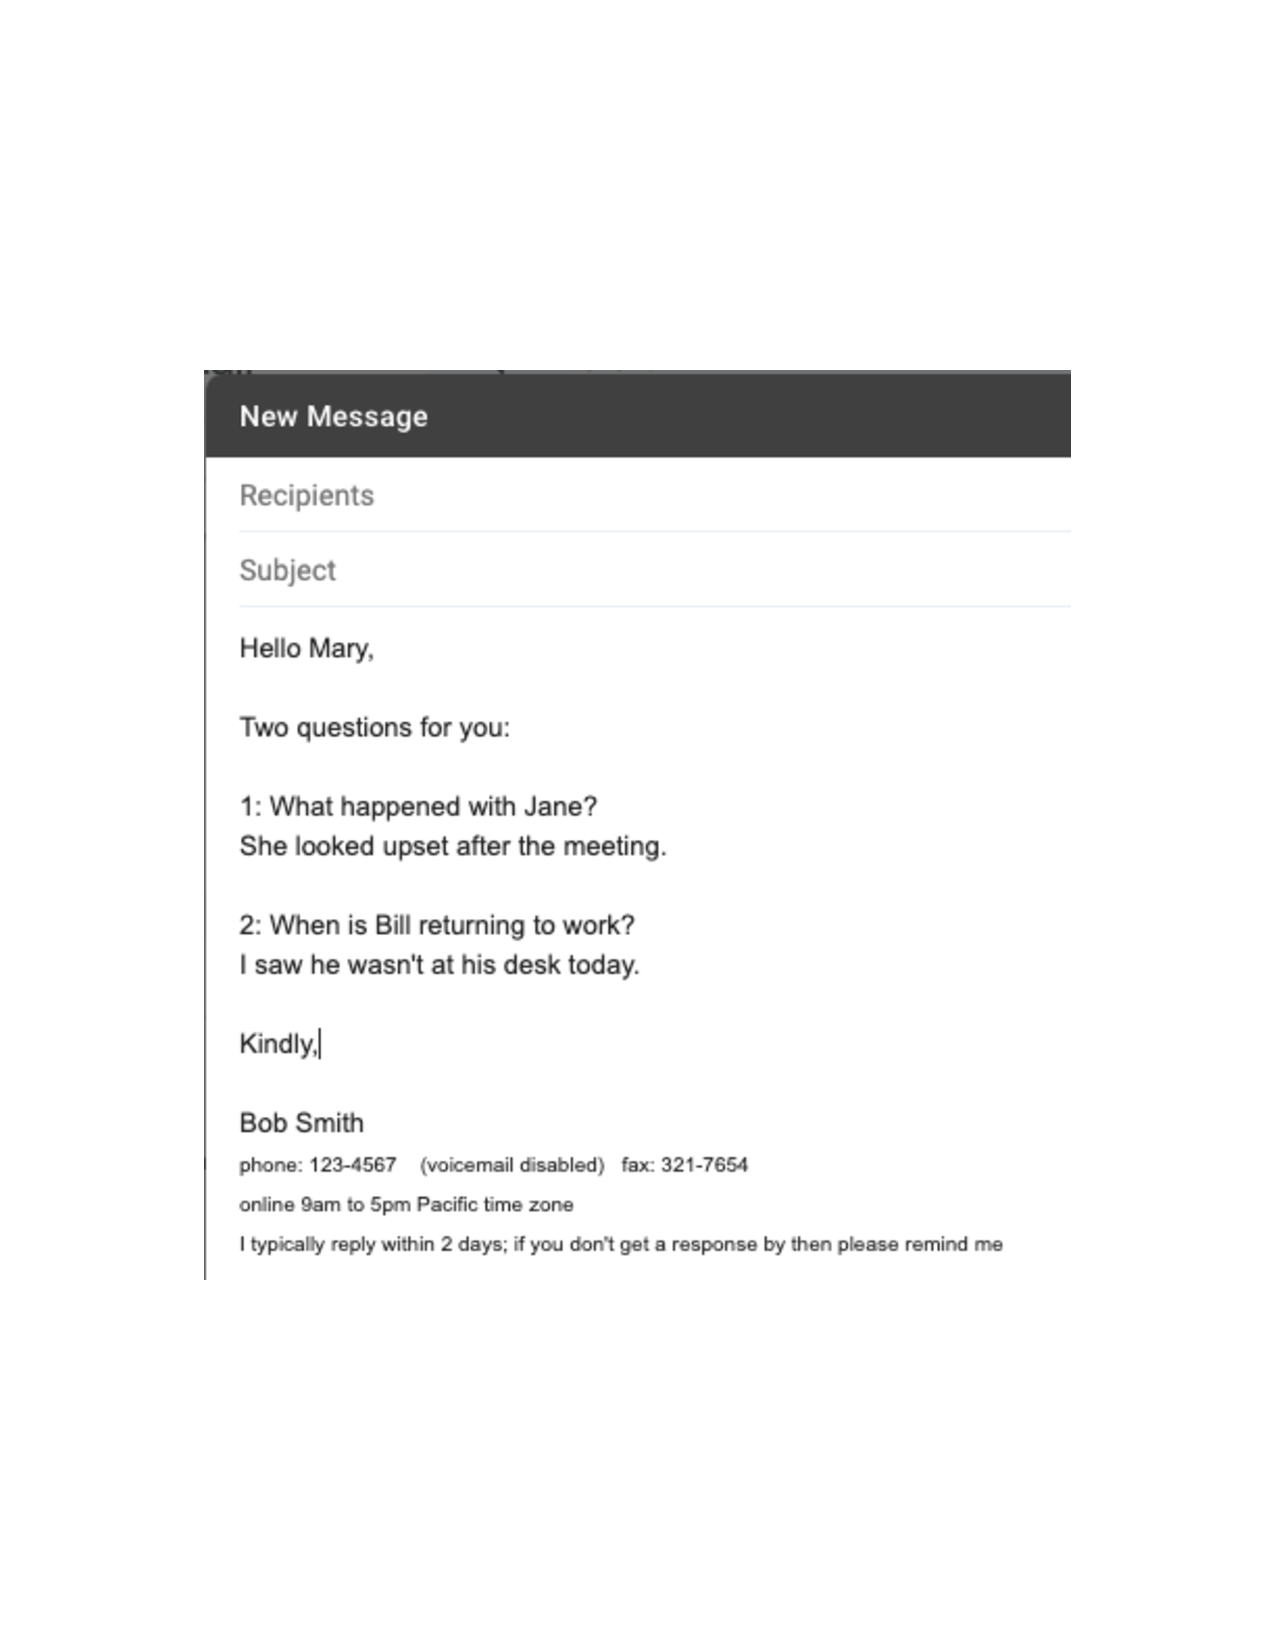
\includegraphics[width=1\textwidth]{images/email_two_questions.pdf}
\caption{Distinct items the recipient should address in a reply.}
\label{fig:email_two_questions}
\end{figure}

If an item corresponds to a requested action, separately highlight the action and indicate who is supposed to take the action and what the deadline for response is.

\begin{figure}
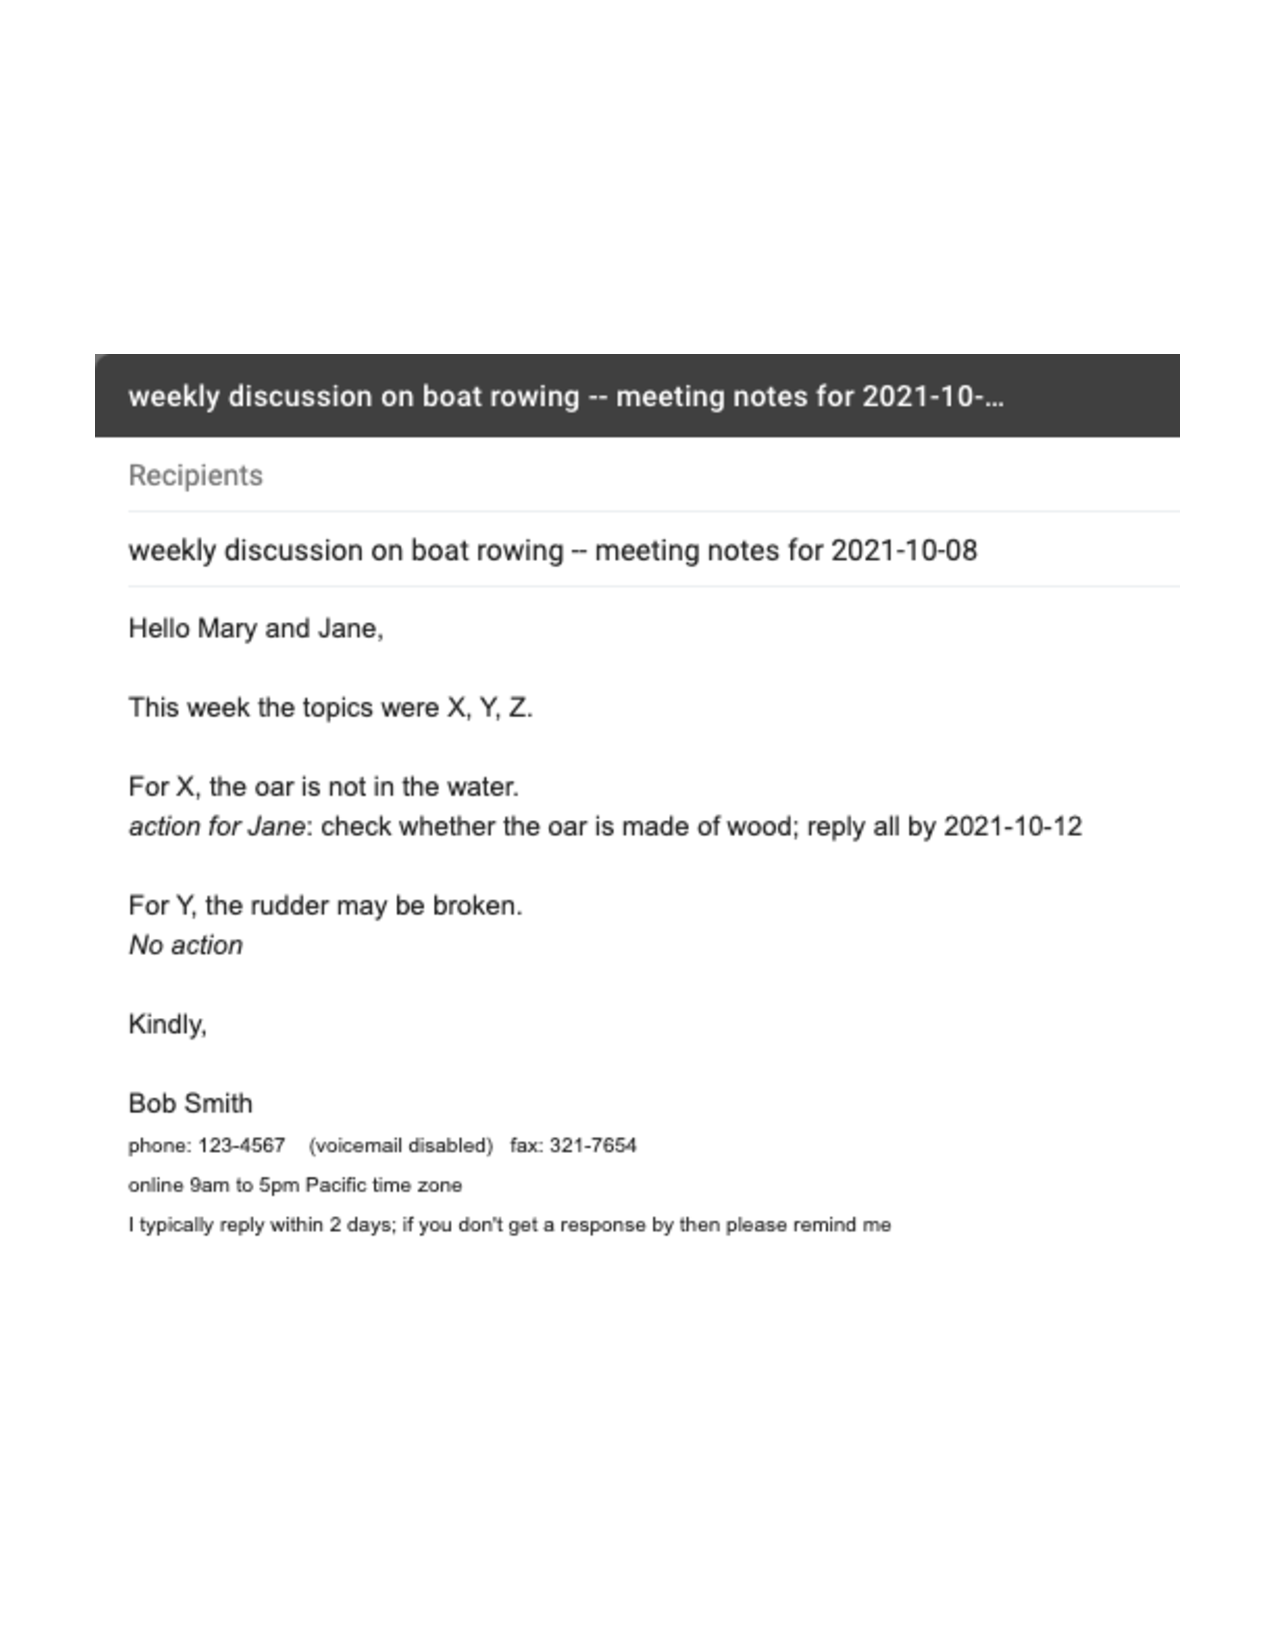
\includegraphics[width=1\textwidth]{images/email_meeting_notes.pdf}
\caption{Who has what action due when?}
\label{fig:email_meeting_notes}
\end{figure}

Computer commands should be distinct separate fixed-width font. This distinguishes the text from the rest of the narrative. 


\begin{figure}
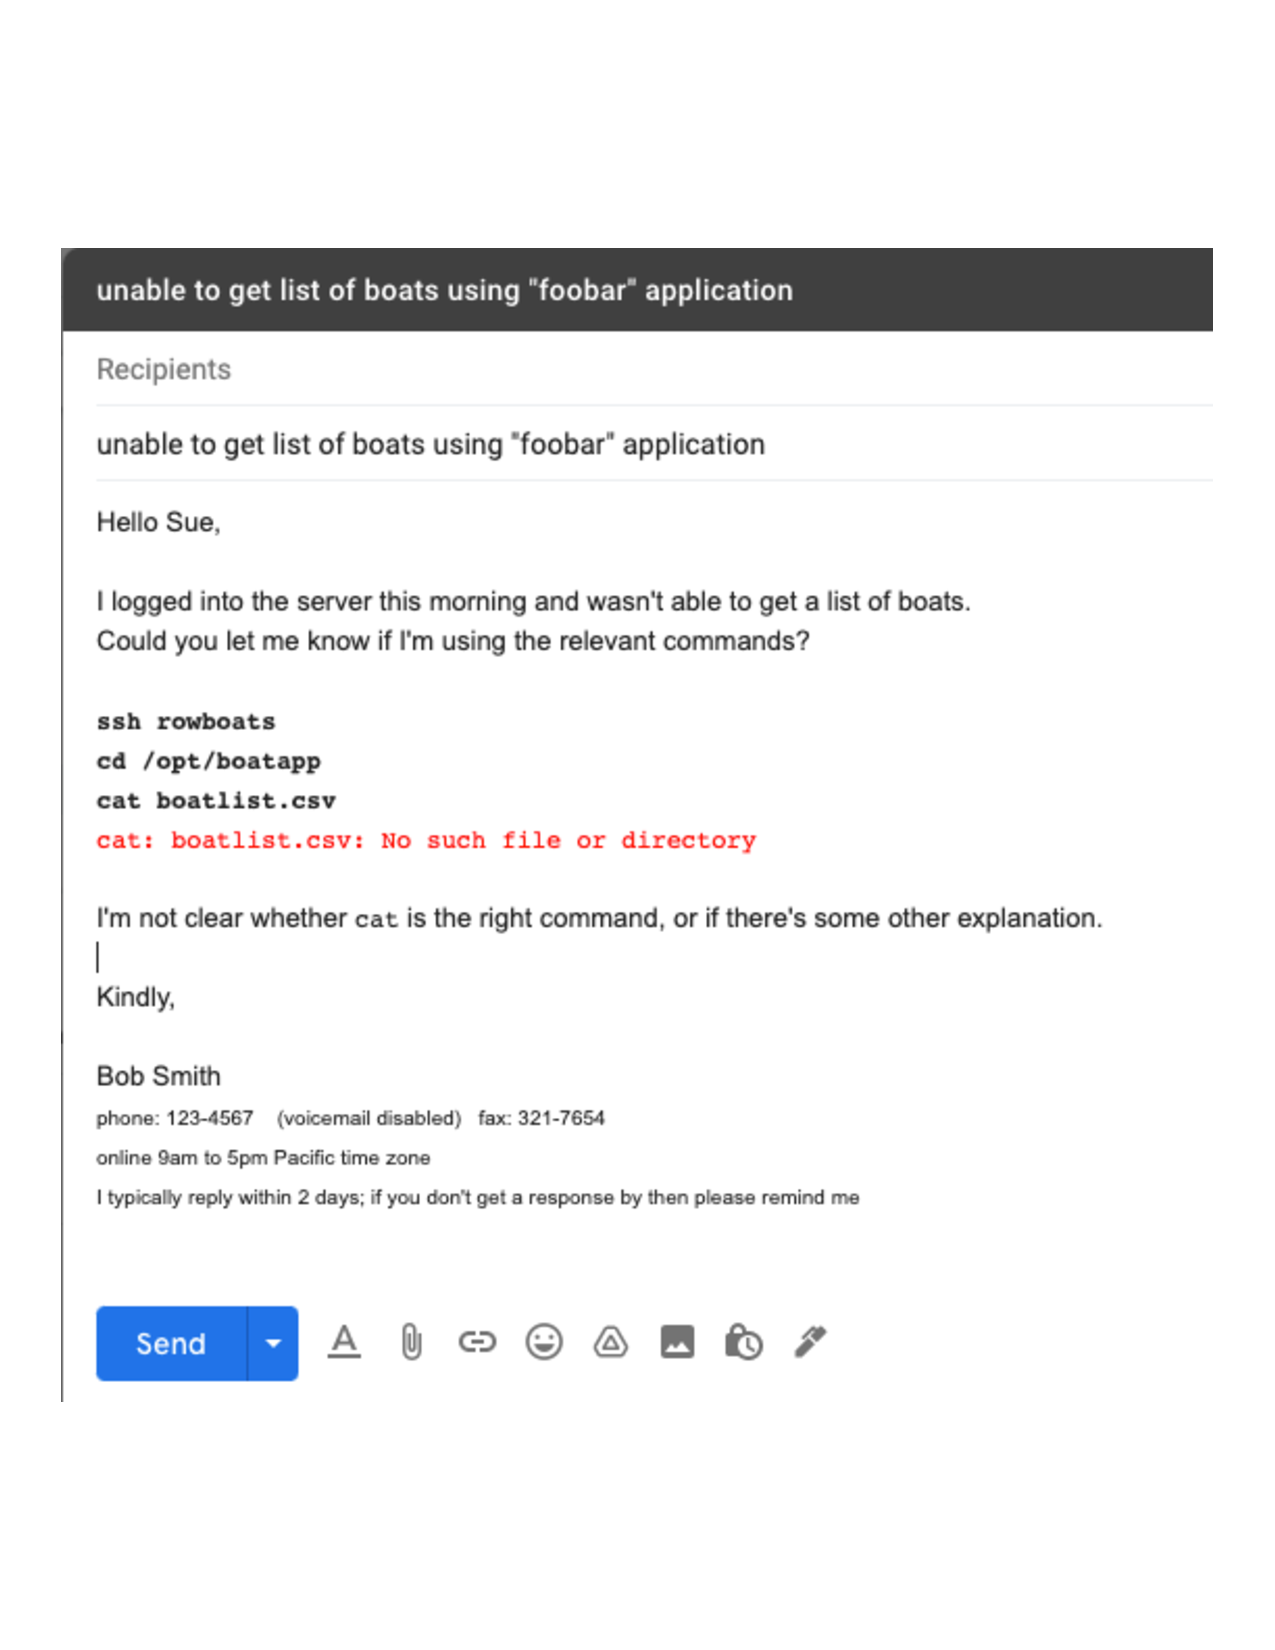
\includegraphics[width=1\textwidth]{images/email_computer_font.pdf}
\caption{The computer commands use fixed width font. The author distinguished input from output through the use of bold vs non-bold respectively. The author highlighted the error message using red. Inline text like ``cat'' in the last line is also fixed width.}
\label{fig:email_computer_font}
\end{figure}

References to documents include a direct full path.

If referring to a previous separate thread, include the subject and the date+time that email was sent

For bullet points, explicitly specify that items are joined by one of the following: OR, XOR, AND

If you have an unordered list, explicitly state that order is irrelevant.

If you have a sequence of steps, number them appropriately and indicate which steps are required versus optional

Use visual sketches to illustrate concepts rather than always relying on text. Don't use pictures all the time, and don't have too many pictures in an email. 

Know how to both embed pictures inline and how to attach files and when to use which. 
Email replies should preferentially be at the top of the thread. 
If replying to multiple points in the previous email, embed replies inline, mark the distinction, and highlight the authorship. 

\begin{figure}
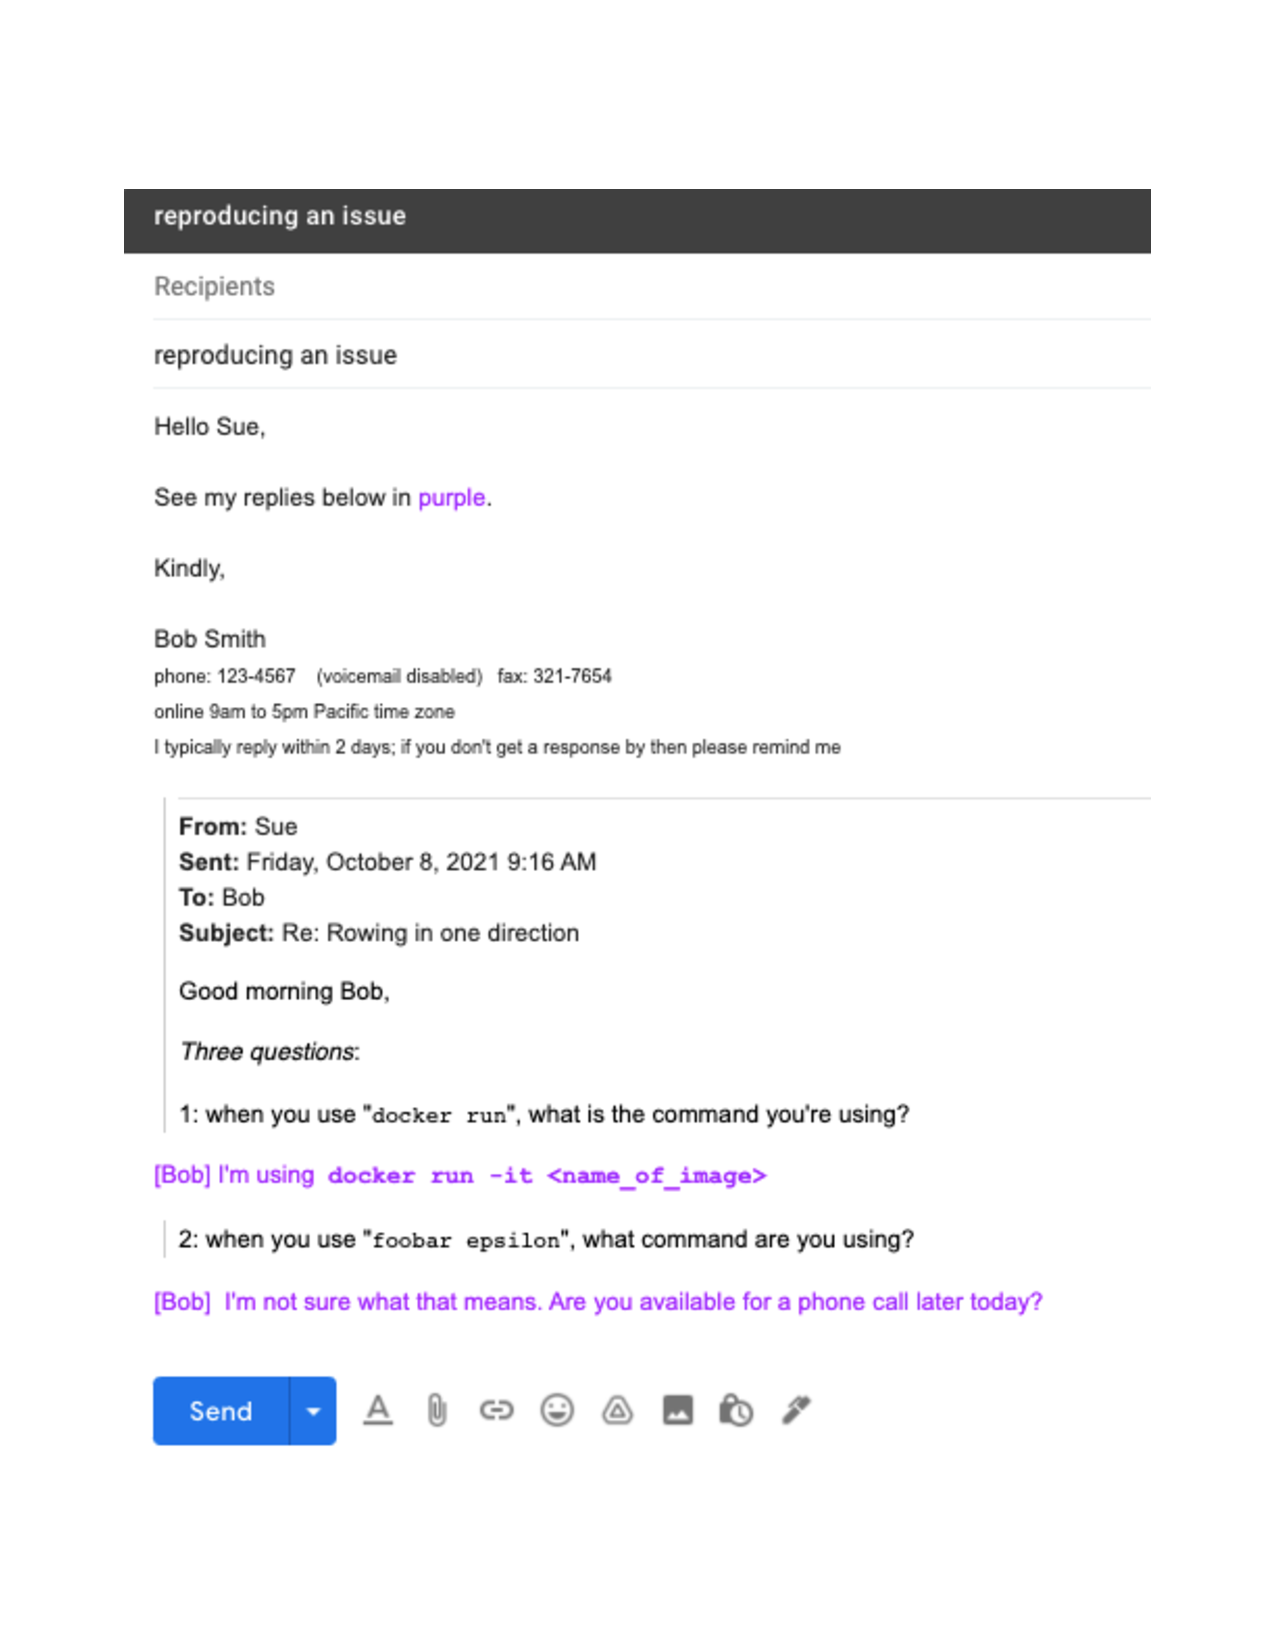
\includegraphics[width=1\textwidth]{images/email_reply.pdf}
\caption{Bob's reply to Sue's questions. The third question is not shown in this illustration.}
\label{fig:email_reply}
\end{figure}

If replying inline, explicitly state that at the top of the thread.

The email trilemma is to balance the amount of detail against providing sufficient context and being concise. 

If the email is longer than a paragraph, provide a \href{https://en.wikipedia.org/wiki/BLUF_(communication)}{B.L.U.F} or \href{https://en.wikipedia.org/wiki/Wikipedia:Too_long;_didn\%27t_read}{tl;dr} or summary. In general emails should be short. Longer discussions should be held on the phone or in person, with a summary report after the discussion. Reliance on a BLUF or tl;dr risks resulting in the reader skipping the content. 

Emails convey both emotional tone and facts. Your intent is practically irrelevant; the reader's perception is paramount. 

Every email should have a purpose. What are you asking the recipient to do? How do you want them to feel? How should they respond?

When replying, starting your email with an expression of gratitude for the work the recipient has done so far sets a positive tone by acknowledging their investment.

\ \\

\subsection*{Summary of what action should be carried out} 

As the outsider, you should help the community enumerate and document all of the problems they identify. Then you can help enumerate and document how the problems are related (dependencies). Only then can you help the community identify and document the root causes.

If the solution you, the outsider, identified really is the root cause, then the community will arrive at that independently. If that is the case, then you can enable them to implement a solution which addresses the root causes. The community will then have a sense of ownership.
